% ====================================================================
% JMP_seminar_beamer_v16.tex -- seminar deck, rebuilt from V15 content.
%
% A REBUILD, not an edit of JMP_seminar_deck_r6.tex (which is kept intact).
% Content comes only from reports/JMP_research_story_report_v15.html and
% reports/JMP_results_gallery_v15.html.  Every numeral is a macro from
% deck_numbers_v16.tex, generated by `make_deck_numbers_r6.py --v16` from
% reports/numbers_of_record_v15.json.  Figures are the V15 image files,
% included unchanged from manuscript/figures/.  Gates: `verify_deck_r6.py
% --deck v16`.  Build: `build_deck_v16.py`.
%
% Presentation boundary: EA is shown first as the opportunity-prospect
% perspective and ATT as the attained-bundle benchmark.  That is an order of
% presentation only; neither perspective is designated primary.
% ====================================================================
\documentclass[10pt,aspectratio=169]{beamer}
% ====================================================================
% jmp_beamer_preamble.tex --- shared preamble for the JMP seminar deck.
%
% REUSED VERBATIM from the companion theory talk
%   beamer/reference/Theory_talk/slides/Presentation.tex
%     "Jobs and Well-Being Measurement" (Haydar and Maniquet)
% so that the two decks read as one visual family.  The elements carried
% over unchanged are marked [THEORY-TALK] below; everything else is an
% addition this deck needs and the theory talk does not.
%
% Consistency is the point: same class options, same theme, same accent
% colour, same frame numbering, same appendix handling, same visible-link
% convention, same note-page template, same two-agent sketch palette.
% ====================================================================

% ---- [THEORY-TALK] class, theme and the deep-red accent -------------
\usetheme{metropolis}
\definecolor{deepred}{RGB}{150,25,35}
\setbeamercolor{frametitle}{bg=deepred}
\setbeamertemplate{navigation symbols}{}
% metropolis-defined accents (safe: these beamercolors exist in metropolis)
\setbeamercolor{progress bar}{fg=deepred}
\setbeamercolor{title separator}{fg=deepred}
% frame number as current/total, in deep red
\metroset{numbering=fraction}
\setbeamercolor{footline}{fg=deepred}
% backup appendix: keep the main frame total at the running-order count
\usepackage{appendixnumberbeamer}
% VISIBLE link colours for rehearsal (internal hyperlinks in deep red)
\hypersetup{colorlinks=true,linkcolor=deepred,citecolor=deepred,urlcolor=deepred}

% ---- [THEORY-TALK] encoding, language, maths, tables, tikz ----------
\usepackage[utf8]{inputenc}
\usepackage[english]{babel}
\usepackage{amsmath}
\usepackage{amssymb}
\usepackage{amsfonts}
\usepackage{booktabs}
\usepackage[official]{eurosym}   % \euro --- this deck quotes euro magnitudes
\usepackage{tikz}
\usetikzlibrary{decorations.pathreplacing,arrows.meta,positioning,fit,backgrounds}

% ---- [THEORY-TALK] the two-agent sketch palette --------------------
% red = agent i / household A ; blue = agent h / household B
\definecolor{agenti}{RGB}{200,30,40}
\definecolor{agenth}{RGB}{20,80,200}

% ---- [THEORY-TALK] notes on a second screen (rehearsal view) -------
% The rehearsal build turns this on; the projection build leaves it off.
\usepackage{pgfpages}
% Long notes overflow the note column by default; render them smaller,
% ragged-right, with tight paragraph spacing so the full text stays
% legible and inside the frame on the second screen.
%
% This deck's notes are longer than the theory talk's -- several run past
% one note page at \scriptsize and produced overfull \vbox warnings.  The
% template below keeps the theory talk's look and adds two things it
% needs: \tiny with a tighter baseline, and an \allowbreak-friendly
% vertical box so a long note breaks across note pages instead of
% overflowing.  Hyphenation is relaxed so no line runs into the margin.
\setbeamertemplate{note page}{%
  \vspace{0.3em}\par
  {\tiny\setlength{\parskip}{0.45em}\setlength{\parindent}{0pt}%
   \setlength{\emergencystretch}{3em}%
   \linespread{1.05}\selectfont
   \raggedright\insertnote\par}%
}
% Notes are prose, not code: let TeX hyphenate freely rather than push a
% long word past the measure.
\hyphenpenalty=50
\tolerance=2000

\DeclareMathOperator*{\argmax}{arg\,max}

% ====================================================================
% ADDITIONS for this deck (not in the theory talk)
% ====================================================================

% ---- channel colours ------------------------------------------------
% One colour per decomposition channel, used consistently on every slide
% that names a channel.  Preferences take the theory talk's agent-red so
% the two decks agree on which side of the argument is which.
\definecolor{chpref}{RGB}{200,30,40}     % preferences   (= agenti)
\definecolor{chacc}{RGB}{20,80,200}      % job access    (= agenth)
\definecolor{chearn}{RGB}{200,120,20}    % earning opportunities
\definecolor{chneeds}{RGB}{40,120,70}    % endowments and needs
\definecolor{chenv}{RGB}{60,60,70}       % the whole environment

% ---- the paper's notation ------------------------------------------
% Audience-facing channel names are WORDS on the slides; these commands
% exist so the words are spelled the same way every time they appear.
\newcommand{\pref}{\textcolor{chpref}{preferences}}
\newcommand{\Pref}{\textcolor{chpref}{Preferences}}
\newcommand{\acc}{\textcolor{chacc}{job access}}
\newcommand{\Acc}{\textcolor{chacc}{Job access}}
\newcommand{\earn}{\textcolor{chearn}{earning opportunities}}
\newcommand{\Earn}{\textcolor{chearn}{Earning opportunities}}
\newcommand{\needs}{\textcolor{chneeds}{household endowments and needs}}
\newcommand{\Needs}{\textcolor{chneeds}{Household endowments and needs}}
\newcommand{\env}{\textcolor{chenv}{the environment}}
\newcommand{\Env}{\textcolor{chenv}{The environment}}

% Symbols.  The theory-paper symbols W, z, R, A, y appear ONLY where the
% companion paper is cited; the estimation notation is separate.
\newcommand{\Wmeasure}{W}                      % theory-paper measure
\newcommand{\Jset}{\mathcal{J}}                % theory-paper job space
\newcommand{\Wone}{W^{1}}                      % theory-paper W^1
\newcommand{\yref}{\mathbf{y}^{w}}             % theory-paper reference pay
\newcommand{\gopp}{g}                          % estimated offer density
\newcommand{\uutil}{u}                         % preference index
\newcommand{\Wmm}{\mathrm{W}}                  % money-metric welfare level

% ---- headline / caveat call-outs -----------------------------------
\newcommand{\headline}[1]{{\large\textcolor{deepred}{#1}}}
\newcommand{\caveat}[1]{{\footnotesize\textcolor{deepred}{#1}}}
% a number with its numerical-integration band
\newcommand{\wband}[2]{#1\,\ensuremath{\pm}\,#2}

% ---- the 25-minute variant ------------------------------------------
% Every frame carries \shortdeck (in the 25-minute running order) or
% \longdeck (45-minute only).  \DeckShort, set by the driver file, drops
% the \longdeck frames; the default keeps everything.
%
% The frozen plan's 25-minute running order is 16 slides, reached from the
% 23 by FIVE cuts and TWO merges:
%   CUT   -> backup : 9, 12, 17, 18, 22          (\longdeck)
%   MERGE           : 6+7 -> one slide, 10+11 -> one slide
% So three tags, not two.  A merged pair is written as two full frames for
% the 45-minute deck; in the short deck the SECOND of the pair drops and
% the first shows its merged content.  23 - 5 - 2 = 16.
%
% Usage:  \shortdeck{\begin{frame}...\end{frame}}     kept in both
%         \longdeck{\begin{frame}...\end{frame}}      45-minute only (cut)
%         \mergedaway{\begin{frame}...\end{frame}}    45-minute only (merged)
%         \ifDeckShort ... \else ... \fi              inline merged content
\newif\ifDeckShort\DeckShortfalse
\newcommand{\shortdeck}[1]{#1}                       % always kept
\newcommand{\longdeck}[1]{\ifDeckShort\else#1\fi}    % cut to backup at 25 min
\newcommand{\mergedaway}[1]{\ifDeckShort\else#1\fi}  % folded into the previous
% content shown only in the merged (25-minute) form of a slide
\newcommand{\mergedonly}[1]{\ifDeckShort#1\fi}

% ---- figure helper ---------------------------------------------------
% Every figure is a PDF from the frozen sprint set, included by name from
% beamer/figures/.  \deckfig{name}{width fraction} keeps the call sites
% uniform and makes a missing file fail loudly at compile time.
\graphicspath{{figures/}}
% Heights leave room for the frametitle, the one caption line every figure
% slide carries, and the metropolis footline -- a taller box overflows the
% frame and shows up as an overfull \vbox.
\newcommand{\deckfig}[2]{%
  \begin{center}\includegraphics[width=#2\textwidth,height=0.70\textheight,%
    keepaspectratio]{#1}\end{center}}
\newcommand{\deckfigtwo}[4]{%
  \begin{columns}[c,onlytextwidth]
  \column{0.49\textwidth}\includegraphics[width=\textwidth,height=0.60\textheight,%
    keepaspectratio]{#1}\\{\centering\scriptsize #2\par}
  \column{0.49\textwidth}\includegraphics[width=\textwidth,height=0.60\textheight,%
    keepaspectratio]{#3}\\{\centering\scriptsize #4\par}
  \end{columns}}

% ---- tables ---------------------------------------------------------
% Several slides carry a comparison table that is naturally wider than the
% text block.  \decktable shrinks one to the measure rather than letting it
% run into the margin (an overfull \hbox), and never enlarges a narrow one.
\newcommand{\decktable}[1]{%
  \begin{center}\resizebox{\textwidth}{!}{#1}\end{center}}

\endinput

\usepackage{array}
\input{deck_numbers_v16}
\graphicspath{{../manuscript/figures/v13/}{../manuscript/figures/v11/}{../manuscript/figures/v5/}}
\metroset{sectionpage=none}
\ifdefined\RehearsalDeck
  \setbeameroption{show notes on second screen=right}
\fi
\newcommand{\presenternotesize}{\small}
\setbeamertemplate{note page}{%
  \vspace{0.3em}\par
  {\presenternotesize\setlength{\parskip}{0.45em}\setlength{\parindent}{0pt}%
   \setlength{\emergencystretch}{3em}\linespread{1.05}\selectfont
   \raggedright\insertnote\par}}
\setbeamerfont{frametitle}{size=\normalsize,series=\bfseries}
\setbeamertemplate{frametitle}{%
  \nointerlineskip
  \begin{beamercolorbox}[wd=\paperwidth,sep=0pt]{frametitle}%
    \vskip0.65em
    \hspace*{1.2em}\begin{minipage}{0.91\paperwidth}%
      \raggedright\hyphenpenalty=10000\exhyphenpenalty=10000
      \insertframetitle\par
    \end{minipage}\par
    \vskip0.65em
  \end{beamercolorbox}}
\renewcommand{\caveat}[1]{{\fontsize{8.2}{10}\selectfont\raggedright\color{deepred}#1\par}}
% channel words, V15 vocabulary
\newcommand{\Pch}{\textcolor{chpref}{preferences}}
\newcommand{\Ach}{\textcolor{chacc}{local access}}
\newcommand{\Bch}{\textcolor{chearn}{earning opportunities}}
\newcommand{\Dch}{\textcolor{chneeds}{household resources, needs and composition}}
\newcommand{\EA}{\textcolor{chacc}{\textbf{EA}}}
\newcommand{\ATT}{\textcolor{chearn}{\textbf{ATT}}}

\title{Unequal Job Opportunities and Well-Being Inequality: A Latent-Jobs Structural Decomposition}
\author{Hisham Haydar}
\date{}

\begin{document}

% ------------------------------------------------------------------ 1 title
\begin{frame}[plain]
\vfill
{\LARGE\bfseries\inserttitle\par}
\vspace{1.3em}
{\color{deepred}\rule{0.80\textwidth}{1pt}}\par
\vspace{1.3em}
{\large Hisham Haydar\par}
University of Luxembourg and LISER\par
\vspace{1.3em}
{\small France: EU-SILC collected in \VCollectionYear{}, incomes of \VIncomeYear{}, every job priced through EUROMOD.\par}
\vspace{0.6em}
{\footnotesize Discussion draft. The decomposition is preliminary and is not a causal decomposition.\par}
\vfill
\note{Thank you. This talk asks how much of the inequality in money-metric
well-being goes with unequal job opportunities rather than with differences in
what people prefer. I will build the answer in four steps: a model of labour
supply as choice among latent jobs, which separates preferences from
opportunities; two ways of turning choices into euros of well-being; a set of
counterfactuals that equalise one source of heterogeneity at a time; and a
Shapley rule that allocates the change. The punchline is that the answer
depends on the welfare question you ask.}
\end{frame}

% ------------------------------------------------------------------ 2 real-world inequality
\begin{frame}
\headlineframe{Two households with the same income can be very differently placed.}
\vfill
\begin{itemize}\itemsep0.55em
  \item Low earnings can mean a taste for short hours, no well-paid job within
        reach, or household resources that make another arrangement affordable.
  \item An income distribution records outcomes with these explanations
        already mixed in.
  \item In France, well-being inequality differs from consumption inequality:
  \begin{itemize}\itemsep0.25em
    \item single adults: consumption Gini \VCEqGiniSingles{}, attained-bundle well-being Gini \VAttEqGiniSingles{};
    \item couples: consumption Gini \VCEqGiniCouples{}, attained-bundle well-being Gini \VAttEqGiniCouples{}.
  \end{itemize}
\end{itemize}
\vfill
\caveat{Equivalised, household-weighted, within each population. Single-adult
and couple households are separate populations and are not compared with each
other.}
\note{Two people can work the same hours for the same hourly pay and be very
differently placed. One chose that job from several that were open; the other
took the only offer available. Their incomes are identical and their
circumstances are not. The Ginis on the slide make the point in the data: once
the leisure a job costs is valued, the dispersion of well-being is not the
dispersion of consumption. These are within-sample dispersion comparisons,
not welfare-loss estimates. The rest of the talk asks which sources of
heterogeneity that well-being inequality goes with.}
\end{frame}

% ------------------------------------------------------------------ 3 literature gap
\begin{frame}
\headlineframe{Each ingredient exists; a decomposition of the level of well-being inequality across them does not.}
\vfill
\begin{columns}[T]
\begin{column}{0.32\textwidth}
{\bfseries Labour supply as choice among latent jobs}\par\smallskip
{\footnotesize Aaberge, Dagsvik and Str{\o}m; Dagsvik and Str{\o}m; Dagsvik and
Jia; Cap\'eau, Decoster and Dekkers.\par\smallskip
Separates tastes from opportunities; used to evaluate \emph{reforms}.\par}
\end{column}
\begin{column}{0.32\textwidth}
{\bfseries Money-metric welfare with heterogeneous preferences}\par\smallskip
{\footnotesize Fleurbaey and Maniquet; Decoster and Haan; Bargain et al.;
Jia and Thoresen; Jacquet, Jia and Thoresen.\par\smallskip
A reference encodes a normative position; references sit on deterministic
budget sets, or value a \emph{change} between regimes.\par}
\end{column}
\begin{column}{0.32\textwidth}
{\bfseries Decomposing inequality}\par\smallskip
{\footnotesize Shorrocks; Sastre and Trannoy; Creedy and H\'erault; M\"uhlhan.\par\smallskip
Shapley allocation of a \emph{change} between policy, population or time
states.\par}
\end{column}
\end{columns}
\vfill
\caveat{Gap: a cross-sectional \emph{level} of well-being inequality, decomposed
into preferences and job opportunities inside an estimated latent-jobs model,
under welfare measures that can value opportunities themselves.}
\note{Every ingredient has antecedents, and the contribution is the
combination and the empirical answer. The latent-jobs framework, with its
excluded opportunity shifters, is due to Aaberge, Dagsvik and Str{\o}m and was
set out for applied work by Cap\'eau, Decoster and Dekkers, who already cover
singles and couples. Money-metric evaluation with such models exists, but it
evaluates a change between policy regimes; our object is a distribution of
levels under one policy system. The normative literature following Fleurbaey
and Maniquet shows how a reference encodes compensation and responsibility.
The closest decompositions, Creedy and H\'erault and M\"uhlhan, decompose a
change between situations. The Shapley rule itself is inherited; no new
allocation principle is claimed.}
\end{frame}

% ------------------------------------------------------------------ 4 research question
\begin{frame}
\headlineframe{Research question}
\vfill
\begin{block}{}
\large How much inequality in money-metric well-being is associated with unequal
job opportunities rather than heterogeneous preferences, once labour supply is
modelled as choice among latent jobs?
\end{block}
\vfill
\begin{enumerate}\itemsep0.45em
  \item Do observed labour-supply choices reflect preferences alone, or also
        heterogeneous latent job opportunities?
  \item How do conclusions differ when welfare evaluates the attained bundle
        versus the ex-ante opportunity prospect?
  \item In a restricted P/A/B decomposition, how much welfare inequality is
        associated with preferences, local access, and earning opportunities?
\end{enumerate}
\vfill
\note{This is the whole talk on one slide. The first subquestion is
behavioural: can we read preferences off choices, or do opportunities get in
the way? The second is normative: once we value well-being in euros, does it
matter whether we value the job a household ends up in or the prospect it
faces? The third is the accounting: inside a restricted decomposition, with
preferences, local access and earning opportunities as the three channels, how
is inequality allocated? Note the word associated: nothing here is causal.}
\end{frame}

% ------------------------------------------------------------------ 5 model: utility
\begin{frame}
\headlineframe{The latent-jobs model: a job is a package, valued through leisure and consumption.}
\vfill
{\small A package $j$: employment, one of four occupation groups, weekly hours and an
hourly wage, priced through the French tax--benefit system to monthly
disposable consumption $C_i(j)$.\par}
\slideeq{$\displaystyle v_i(j)=L_i(j)+\beta_c\log\!\left(\frac{C_i(j)}{\lambda_c}\right)$}
\glossrow{$L_i$ value of leisure, shifted by age and, for women, children
\quad $\beta_c$ weight on log consumption, estimated \quad $\lambda_c$ a units
convention}
\vfill
\caveat{Estimated separately for \VNSingles{} single-adult and \VNCouples{}
couple households. The child term is a reduced-form time-constraint shifter,
not pure taste.}
\note{In words: a household's systematic value of a job is the value of the
leisure it leaves plus the log of the consumption it pays. The split matters
later, because consumption is observable in euros and leisure is not; it is
what turns a utility gap into a proportional consumption adjustment in both
welfare measures. For a couple, the leisure term sums both spouses' terms and
consumption is joint. The household-specific leisure coefficients, age
profiles and the child-related shifter, are the preference channel we later
equalise.}
\end{frame}

% ------------------------------------------------------------------ 6 model: choice law
\begin{frame}
\headlineframe{A job is chosen because it is valued or because it is plentiful: the choice law carries an opportunity density.}
\slideeq{$\displaystyle P_i(j)=\frac{\exp\{v_i(j)\}\,g_i(j)}{\displaystyle\int\exp\{v_i(k)\}\,g_i(k)\,d\nu(k)}$}
\glossrow{$g_i$: how intensely package $j$ is available to household $i$ before
any choice. It has four blocks: \textcolor{chacc}{access} (local unemployment
exposure, region, urban or rural location, year), hours bands, occupation, and
\textcolor{chearn}{wage offers} (education, experience).}
\vfill
\caveat{Separation rests on maintained restrictions: smooth preferences against
banded hours opportunities; local shifters excluded from preferences; wage
offers independent of hours given occupation.}
\note{In words: the probability of being seen in a job is its value times its
availability, normalised over all jobs. If everyone faced the same density, we
would be back to a standard model where every difference in behaviour must be a
difference in taste. Because the density is household-specific, part of
behaviour can be attributed to reachability. A spike at a band of hours is read
as availability, not a kink in tastes; the local unemployment measure and the
geography shift access and appear nowhere in utility. These are maintained
restrictions, not tested ones, and the regional variation is not a causal
design.}
\end{frame}

% ------------------------------------------------------------------ 7 matched households
\begin{frame}
\headlineframe{What unequal opportunity means here: two matched men with almost identical tastes.}
\begin{center}
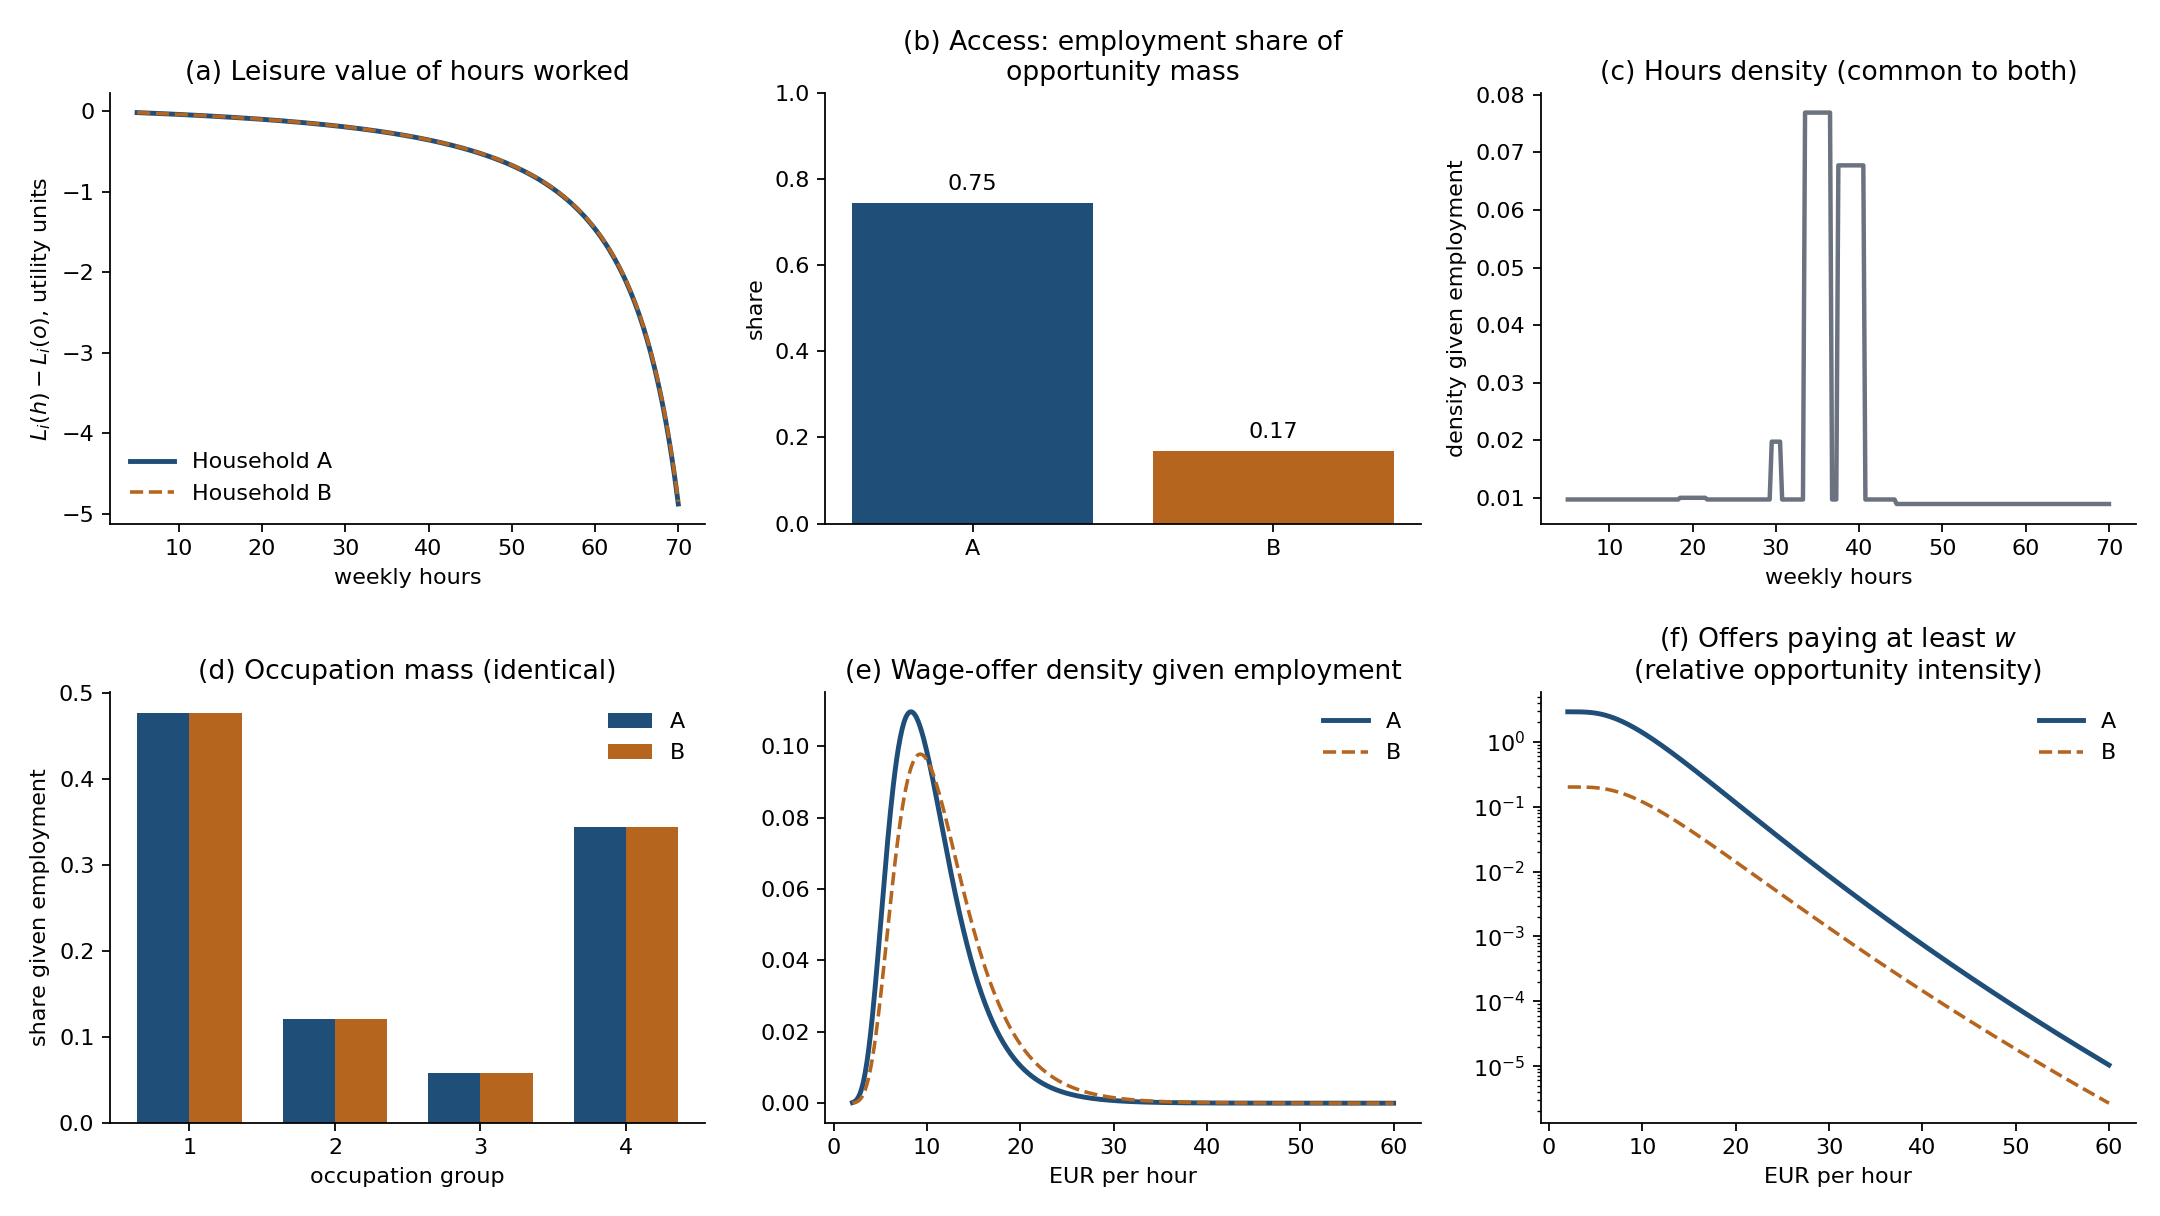
\includegraphics[height=0.66\textheight,width=\textwidth,keepaspectratio]{fig_matched_households_v11.png}
\end{center}
\caveat{Same occupation group, hours band and wage quintile. A has
\VMatchedAccessRatio{} times B's employment mass; B's wage-offer location is
\VMatchedWageGap{} log points higher. A stated-rule teaching example: not
causal, not representative.}
\note{These two single men look alike in an income table and have nearly
identical estimated leisure profiles. If both were indifferent between all
jobs and not working, employment would be \VMatchedEmpShareA{} of A's
opportunity mass and \VMatchedEmpShareB{} of B's; the gap comes from local
unemployment exposure and region. B's wage offers are better, yet A faces more
offers paying at least any given wage over essentially all offer mass. Neither
is better placed on every margin, and which one is better off depends on how
welfare weighs the number of reachable jobs against what the realised job
pays. That is exactly the question that separates the two welfare
perspectives.}
\end{frame}

% ------------------------------------------------------------------ 8 subquestion 1
\begin{frame}
\headlineframe{First subquestion: choices reflect opportunities as well as preferences.}
\vfill
\begin{center}\small
\begin{tabular}{>{\raggedright\arraybackslash}p{0.50\textwidth}cc}
\toprule
Single adults & free coordinates & population fit \\
 & & (mean absolute deviation) \\
\midrule
Latent jobs, household-specific opportunities & \VKFreeSingles{} & \VMaeSingles{} \\
Common opportunity distribution & \VKFreeRumA{} & \VMaeRumA{} \\
Common opportunity shape; employment and hours moved into utility & \VKFreeRumB{} & \VMaeRumB{} \\
\bottomrule
\end{tabular}
\end{center}
\vfill
{\small Both re-estimated common-opportunity benchmarks are worse by at least
\VRumGap{} on the same criterion, households and sampled alternatives; the
occupation margins deteriorate by an order of magnitude.\par}
\vfill
\caveat{Not converted into a formal test. A better criterion does not by itself
establish that a mechanism has been identified.}
\note{The first subquestion. Take away the household-specific opportunity
block, re-estimate everything else, and the model does worse, on the same
households and the same criterion. The deterioration is concentrated where the
opportunity block does its work: population fit roughly doubles its error and
occupation margins deteriorate most. I do not turn this into a likelihood-ratio
test, because the sampled-alternative criterion is not the likelihood of the
observed data. Fit is not perfect either: the observed concentration at exactly
thirty-seven hours is underpredicted in every group, and extensive-margin
accuracy for men is withheld because integration error is too large.}
\end{frame}

% ------------------------------------------------------------------ 9 theory figure
\begin{frame}
\headlineframe{From choices to well-being: give every job the same consumption and ask what is as good as the actual situation.}
\begin{columns}[c]
\begin{column}{0.56\textwidth}
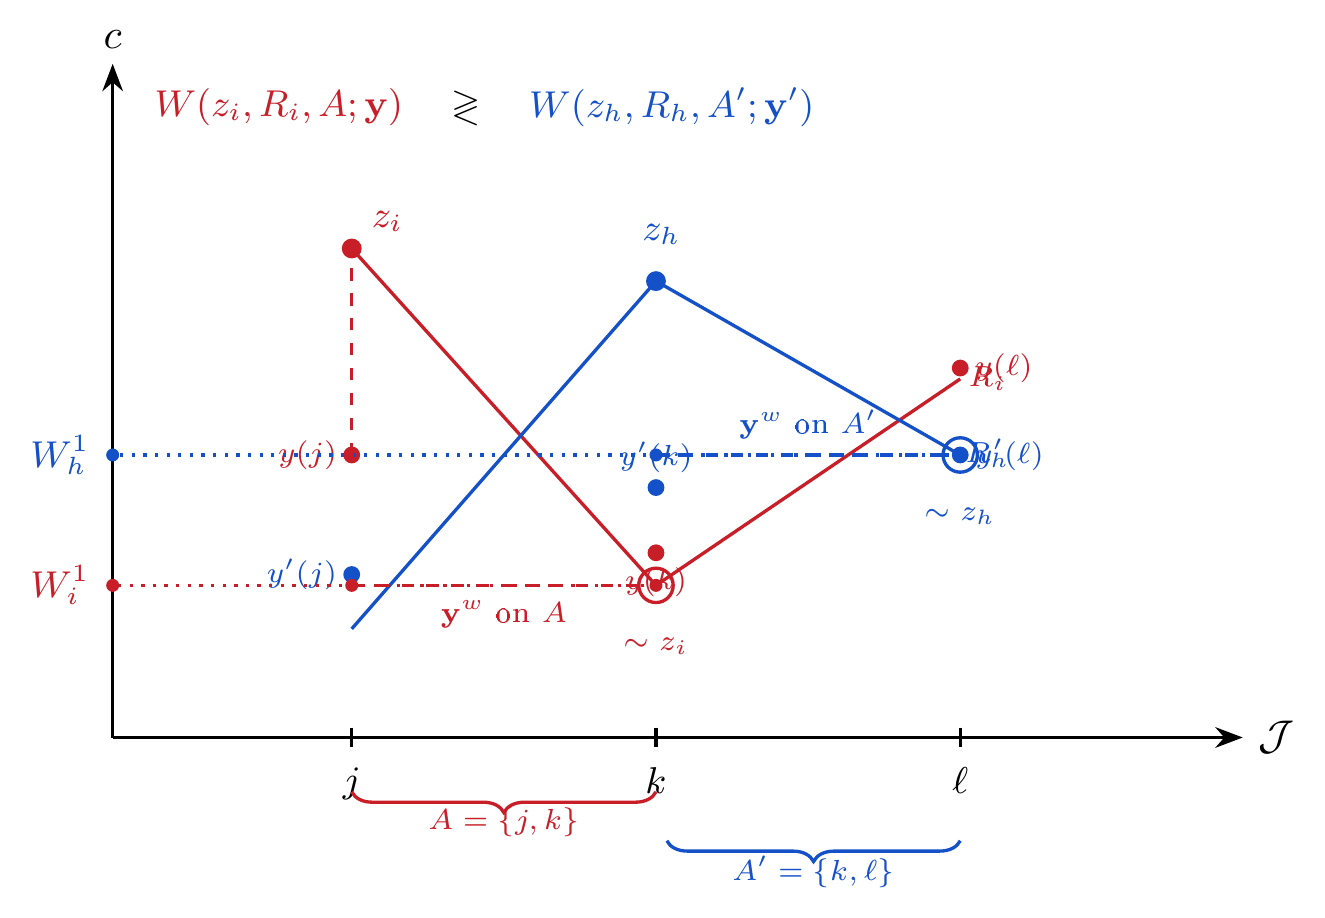
\includegraphics[width=\textwidth,height=0.72\textheight,keepaspectratio]{theory_w1.png}
\end{column}
\begin{column}{0.42\textwidth}
{\scriptsize\raggedright
Own-set equal-consumption equivalents: the theoretical construction from the companion theory paper. Two individuals, with preferences $R_i$ and $R_h$ and ability sets $A=\{j,k\}$ and $A^{\prime}=\{k,\ell\}$, attain bundles $z_i$ and $z_h$. For each individual, a common consumption level is assigned to every job in their own set; the level at which the preferred reference job becomes indifferent to the attained bundle is that individual's money metric, $W^1_i$ and $W^1_h$. The two metrics are then directly comparable. Adapted from Haydar and Maniquet (2026), work in progress. This is the deterministic construction; the estimated ex-ante measure is its extension, defined in Section 3.\par}
\end{column}
\end{columns}
\note{Estimated utility is not an interpersonal welfare index: preferences
differ, so the same utility number means different things for different
people. Both money metrics descend from this construction. Each individual is
evaluated with their own preferences and their own set of jobs. Give every job
in that set the same consumption; the individual then prefers one of them, and
the consumption at which that job is exactly as good as the attained bundle is
their money metric. The point is that these metrics are comparable across
people whose preferences and job sets differ. The figure is a theoretical
illustration with no estimated value in it. The choice of reference is the
welfare question, and the next two slides ask two.}
\end{frame}

% ------------------------------------------------------------------ 10 EA
\begin{frame}
\headlineframe{EA, the opportunity-prospect perspective: what flat consumption makes the whole job prospect equally valuable?}
\slideeq{$\displaystyle\begin{gathered}
  J_i=\int e^{L_i(j)}\Big(\tfrac{C_i(j)}{\lambda_c}\Big)^{\beta_c}\,\widehat g_i(j)\,d\nu(j),
  \qquad
  H_i=\int e^{L_i(j)}\,\widehat g_i(j)\,d\nu(j),
  \\[0.35em]
  M^{\mathrm{EA}}_i=\lambda_c\exp\!\Big\{\tfrac{\log J_i-\log H_i}{\beta_c}\Big\}
  \end{gathered}$}
\begin{itemize}\itemsep0.25em
  \item {\small $J_i$: the actual prospect; every job enters, weighted by how available it is and how much it is valued.}
  \item {\small $H_i$: the same jobs, availability and preferences, with pay differences removed.}
  \item {\small Opportunities enter welfare directly: access moves which jobs carry weight; earning opportunities move what they pay.}
\end{itemize}
\vfill
\caveat{The measure treats taste-shock variety as part of what makes a rich
prospect valuable: a normative position, not a consequence of estimation.}
\note{In words: EA is the constant monthly consumption at which a prospect with
the household's own jobs and availability, but equal pay everywhere, is worth
exactly as much as the prospect it actually faces. A common rescaling of the
opportunity density cancels, so what matters is how opportunity weight is
spread across jobs. I show this perspective first because this talk is about
opportunities; that is an order of presentation, not a ranking. Under the
extreme-value shocks, log J is the expected utility of the best reachable job
up to a constant, which is why taste-shock variety counts; I flag that as a
normative choice. The ex-ante calculation passed its numerical checks, which
certifies the computation, not the model's assumptions.}
\end{frame}

% ------------------------------------------------------------------ 11 ATT
\begin{frame}
\headlineframe{ATT, the attained-bundle benchmark: what consumption without work is as good as the job actually held?}
\slideeq{$\displaystyle M^{\mathrm{att}}_i=C^{\mathrm{obs}}_i\exp\!\left\{\frac{L_i(j^{\mathrm{obs}}_i)-L_i(o)}{\beta_c}\right\}$}
\begin{itemize}\itemsep0.3em
  \item {\small Reference: non-employment $o$, which every household can reach.}
  \item {\small Opportunities matter only through which job is attained and what it pays; jobs not taken play no role.}
  \item {\small For non-workers $M^{\mathrm{att}}_i=C^{\mathrm{obs}}_i$; for workers it lies below observed consumption by the value of the leisure given up.}
\end{itemize}
\vfill
\caveat{On the current empirical domain the equal-consumption reference job is
non-employment for every household: a verified property of the estimated
specification, not a general theorem.}
\note{In words: ATT is observed consumption, adjusted by the leisure the job
costs relative to not working, converted at the rate one over the consumption
weight. The general construction evaluates the attained bundle against the job
the household would most prefer if all jobs paid the same; here that job is
non-employment for everyone, so the measure coincides with the staying-home
equivalent. Once the job is fixed, the opportunity density has no direct term.
This is the natural benchmark: it values the outcome reached.}
\end{frame}

% ------------------------------------------------------------------ 12 two questions
\begin{frame}
\headlineframe{The two measures answer different welfare questions.}
\vfill
\begin{center}\small
\renewcommand{\arraystretch}{1.25}
\begin{tabular}{>{\raggedright\arraybackslash}p{0.20\textwidth}>{\raggedright\arraybackslash}p{0.35\textwidth}>{\raggedright\arraybackslash}p{0.35\textwidth}}
\toprule
 & \EA{}: the opportunity prospect & \ATT{}: the attained bundle \\
\midrule
Question & How valuable is the distribution of job prospects the household faces? & How well off is the household in the bundle it actually attains? \\
Reference & The same opportunity environment, with consumption equalised across jobs & A common non-employment state \\
How opportunities enter & Directly, as weights on every job & Only through the realised job \\
\bottomrule
\end{tabular}
\end{center}
\vfill
\caveat{Neither perspective corrects the other, and neither is designated
primary. The choice between them is a substantive normative decision that is not
made here.}
\note{This is the hinge of the talk. The attained-bundle measure evaluates the
bundle eventually reached against a common non-employment reference. The
ex-ante measure evaluates the household's entire distribution of potential job
outcomes against a reference prospect that keeps the same opportunity
environment and equalises consumption across jobs. Because opportunities reach
them by different routes, the two can attribute inequality to different
labour-market channels. When they do, the difference tells us what each welfare
question makes visible. It is not a disagreement to be resolved by choosing a
winner.}
\end{frame}

% ------------------------------------------------------------------ 13 decomposition
\begin{frame}
\headlineframe{The decomposition equalises three channels and allocates the change in the Gini over all orders.}
\vspace{0.3em}
\begin{columns}[T]
\begin{column}{0.48\textwidth}
{\small
\textcolor{chpref}{\textbf{P}} \Pch{}: age profiles and the child-related shifter.\par\smallskip
\textcolor{chacc}{\textbf{A}} \Ach{}: local unemployment exposure, region, urban or rural location, year. Not total opportunity.\par}
\end{column}
\begin{column}{0.48\textwidth}
{\small
\textcolor{chearn}{\textbf{B}} \Bch{}: systematic wage-offer location, not wage dispersion.\par\smallskip
\textcolor{chneeds}{\textbf{Held fixed}}: \Dch{}, in every coalition, with no allocated share.\par}
\end{column}
\end{columns}
\slideeq{$\displaystyle\phi^p_k=\sum_{S\subseteq\{P,A,B\}\setminus\{k\}}\frac{|S|!\,(3-|S|-1)!}{3!}\Big[v^p(S\cup\{k\})-v^p(S)\Big]$}
\glossrow{$v^p(S)=I^p(\varnothing)-I^p(S)$: the fall in the household-weighted Gini of welfare $M^p$, $p\in\{\mathrm{EA},\mathrm{att}\}$, when the channels in $S$ are set to a common reference.}
\vfill
\caveat{Household resources, needs and composition are held fixed in the current
decomposition. The access channel is local access, not total opportunity. The
decomposition is preliminary and makes no causal claim.}
\note{In words: a channel's Shapley contribution is its marginal effect on
inequality averaged over every order in which the three equalisations can be
introduced, and the three contributions add up exactly to the total change.
Each coalition is a full structural counterfactual: coefficients are never
changed, welfare is recomputed for every household under each perspective, and
inequality is measured again. The same operators and rule are applied to both
perspectives, which is what makes their orderings comparable. Contributions are
signed: a negative term means equalising that channel raises inequality on
average over orders. Adding resources, needs and composition as a fourth
channel is a planned extension; with it, access plus earnings would still be
the opportunity component, and the broader sum would not be an opportunity
share.}
\end{frame}

% ------------------------------------------------------------------ 14 central result
\begin{frame}
\headlineframe{Central result: earning opportunities dominate under ATT; access dominates under EA for single adults; couples show no reversal.}
\begin{center}
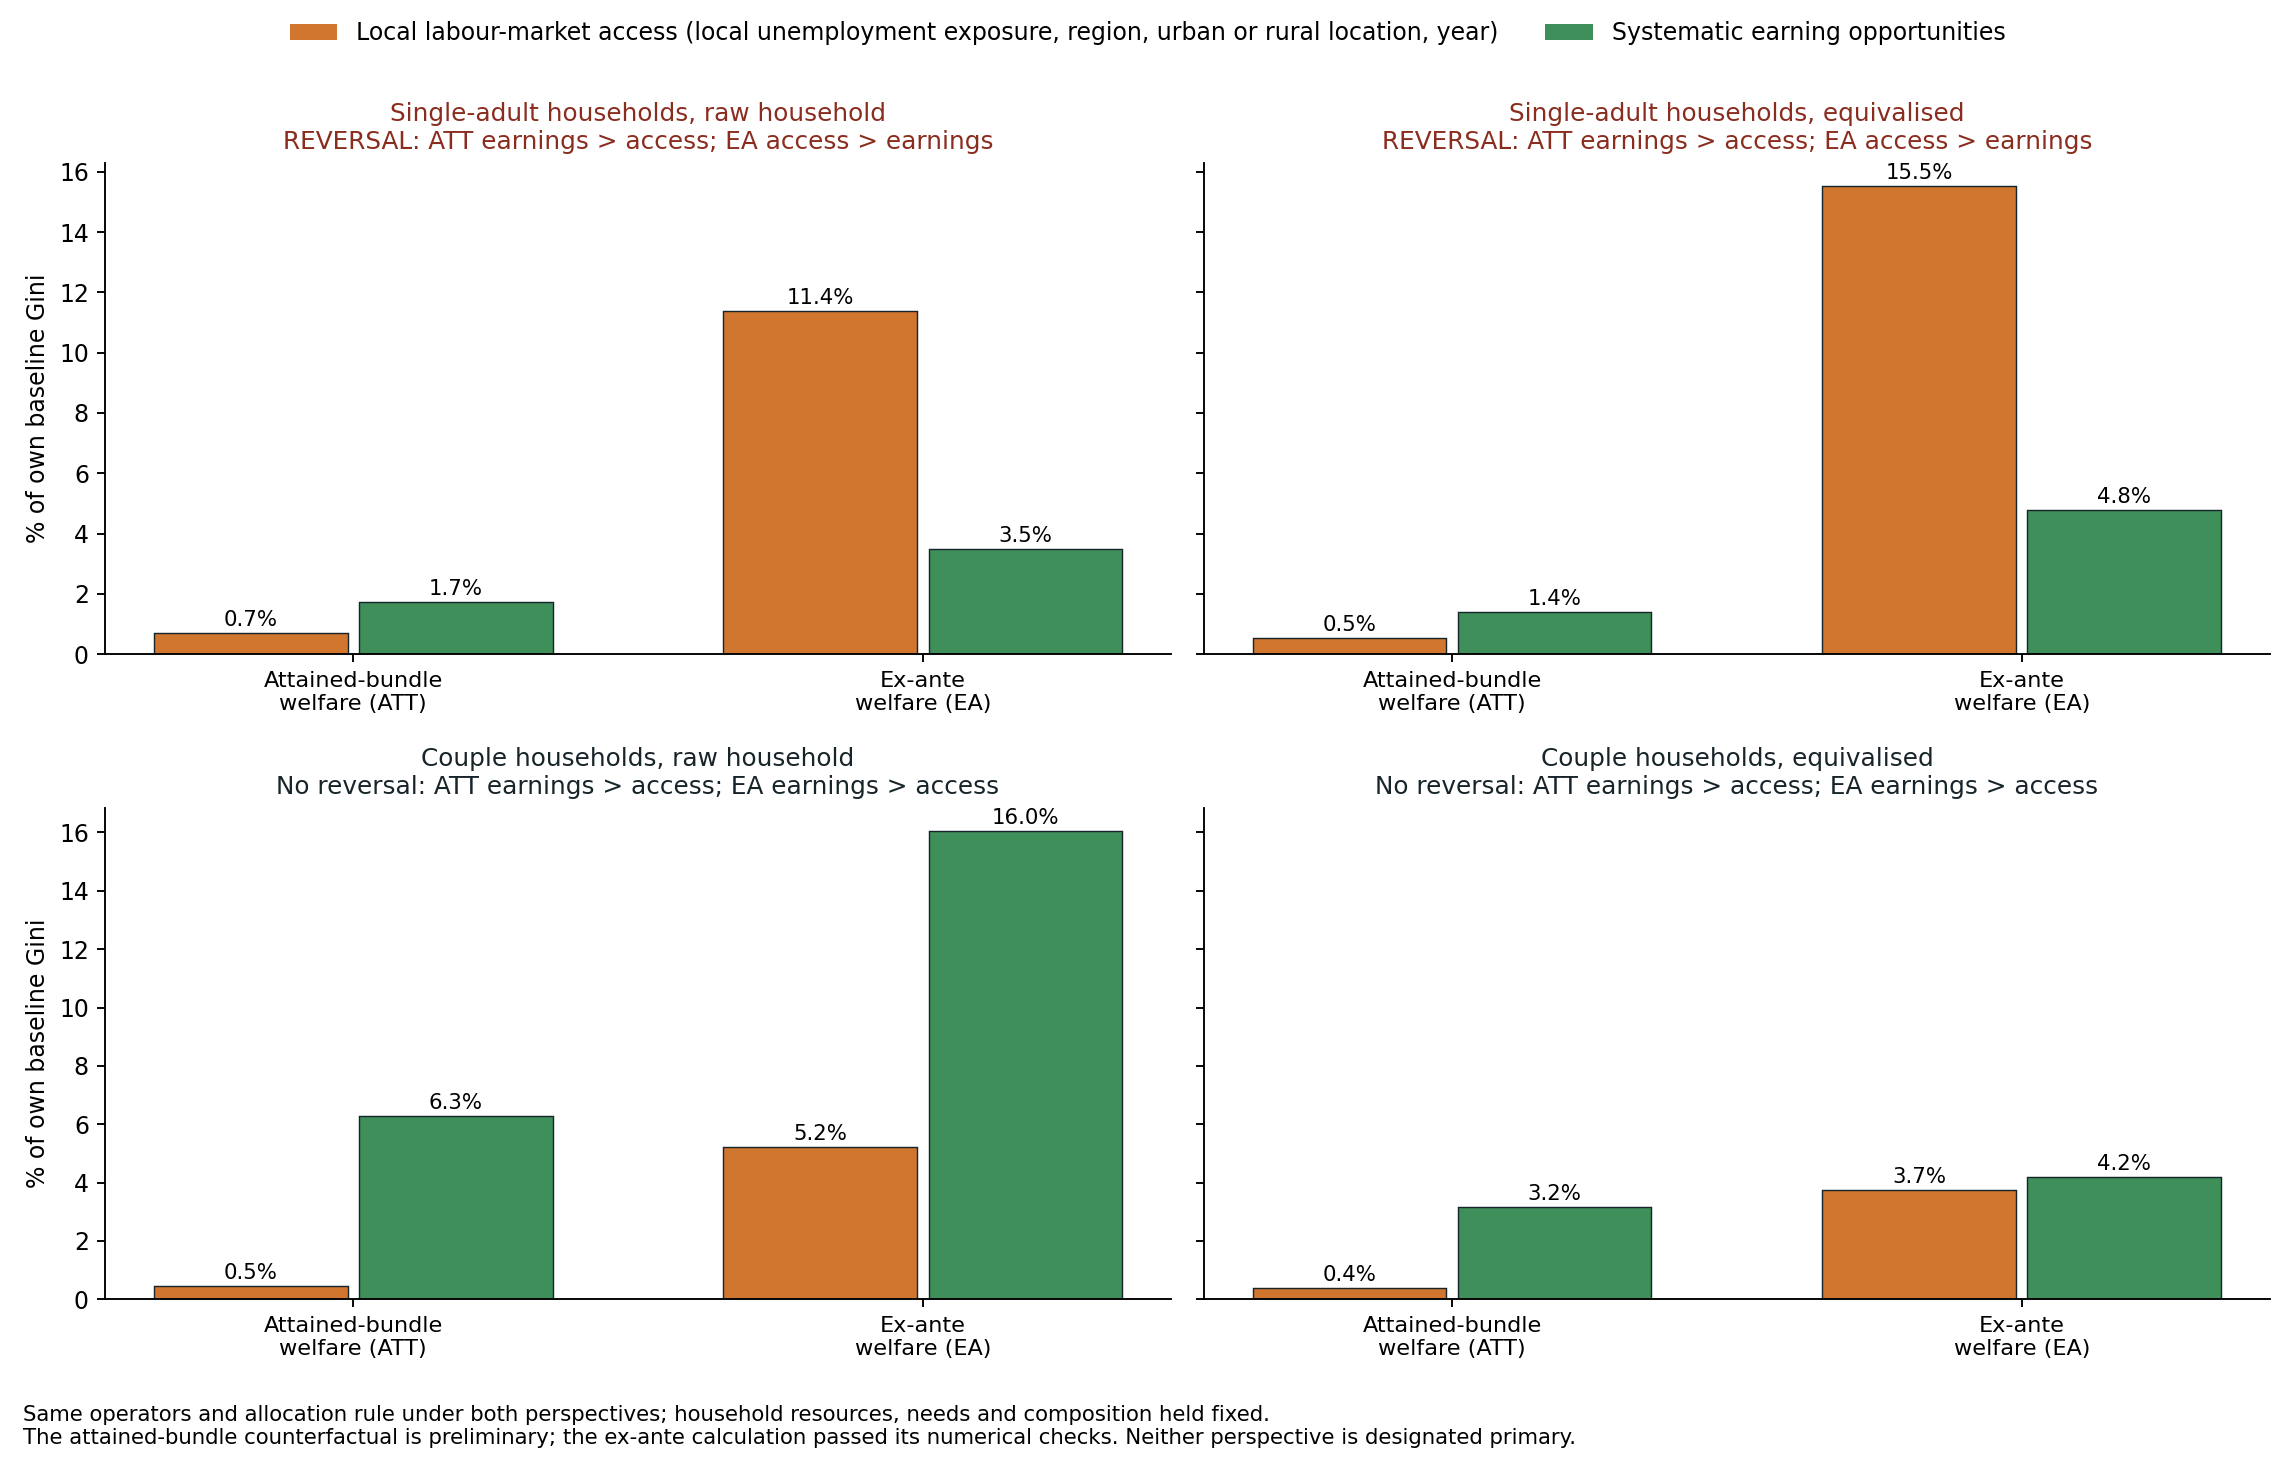
\includegraphics[height=0.60\textheight,width=\textwidth,keepaspectratio]{fig_v13_central_result.png}
\end{center}
\caveat{Access and earning-opportunity contributions as a percentage of each
perspective's own baseline Gini. Access is local access, not total opportunity;
household resources, needs and composition are held fixed. Neither perspective
is designated primary.}
\note{This is the result. Read each panel as the same two operators, local
access and earning opportunities, evaluated under two welfare questions. For
single adults, earning opportunities are the larger channel when we value the
attained bundle, and access is the larger channel when we value the prospect,
on both reporting scales. For couples, earning opportunities stay in front
under both. The mechanism is the route by which opportunities enter: the
attained-bundle measure sees only the realised job, where the wage drives
consumption; the ex-ante measure weights every job by its availability, so the
access environment enters directly. Why single adults reverse and couples do
not is not tested here; one reading is that a single adult's participation
rests on one earner's access. The comparison is also not a pure contrast of
definitions, because the two integrations use different designs.}
\end{frame}

% ------------------------------------------------------------------ 15 EA results
\begin{frame}
\headlineframe{EA: access and earnings account for \VEAOppMin{}--\VEAOppMax{}\% of baseline inequality; for single adults access is about three times earnings.}
\vfill
\decktable{\begin{tabular}{llcccl}
\toprule
 & scale & \textcolor{chacc}{access} & \textcolor{chearn}{earnings} & access + earnings & ordering \\
 & & Gini points & Gini points & \% of baseline & \\
\midrule
Single adults & raw & \VEASingPhiARaw{} & \VEASingPhiBRaw{} & \VEASingOppRaw{} & access $>$ earnings \\
              & equivalised & \VEASingPhiAEq{} & \VEASingPhiBEq{} & \VEASingOppEq{} & access $>$ earnings \\
\midrule
Couples & raw & \VEACoupPhiARaw{} & \VEACoupPhiBRaw{} & \VEACoupOppRaw{} & earnings $>$ access \\
        & equivalised & \VEACoupPhiAEq{} & \VEACoupPhiBEq{} & \VEACoupOppEq{} & earnings $>$ access \\
\bottomrule
\end{tabular}}
\vfill
{\small Single adults: access is \VEASingRatioRaw{} times earnings before
equivalisation and \VEASingRatioEq{} times after it.\par}
\vfill
\caveat{Household resources, needs and composition held fixed; access is local
access. For couples, equivalisation moves the share from \VEACoupOppRaw{}\% to
\VEACoupOppEq{}\% and turns the preference term negative, so no directional
claim about preferences is made.}
\note{The ex-ante numbers. The calculation passed its numerical checks,
including an independent implementation. For couples the scale convention is
substantively consequential: the preference contribution goes from
\VEACoupPrefRaw{} Gini points to \VEACoupPrefEq{} when we equivalise. A negative
Shapley term means that, averaged over orders, equalising preferences raises
inequality; it does not show that preference heterogeneity is equalising in any
causal or welfare sense. That is why both scales are always shown. These are
restricted accounting shares, not the total share of well-being inequality
caused by unequal job opportunities.}
\end{frame}

% ------------------------------------------------------------------ 16 ATT results
\begin{frame}
\headlineframe{ATT benchmark: access and earnings account for \VAttOppMin{}--\VAttOppMax{}\% of baseline inequality, and earning opportunities are larger throughout.}
\vfill
\decktable{\begin{tabular}{llcccl}
\toprule
 & scale & \textcolor{chacc}{access} & \textcolor{chearn}{earnings} & access + earnings & ordering \\
 & & Gini points & Gini points & \% of baseline & \\
\midrule
Single adults & raw & \VAttSingPhiARaw{} & \VAttSingPhiBRaw{} & \VAttSingOppRaw{} & earnings $>$ access \\
              & equivalised & \VAttSingPhiAEq{} & \VAttSingPhiBEq{} & \VAttSingOppEq{} & earnings $>$ access \\
\midrule
Couples & raw & \VAttCoupPhiARaw{} & \VAttCoupPhiBRaw{} & \VAttCoupOppRaw{} & earnings $>$ access \\
        & equivalised & \VAttCoupPhiAEq{} & \VAttCoupPhiBEq{} & \VAttCoupOppEq{} & earnings $>$ access \\
\bottomrule
\end{tabular}}
\vfill
\caveat{Preliminary: the attained-bundle counterfactual integration is still
being validated and covers short hours sparsely. The preference contribution
changes sign with equivalisation in both samples, so no directional claim is
made about it. Household resources, needs and composition held fixed.}
\note{The attained-bundle benchmark. Earning opportunities are larger than
local access for both household types and on both scales. Every coalition Gini
and contribution reproduces closely under an independent simulation run, and
the allocation closes to numerical precision; those checks validate the
calculation for the stated game, not its maintained assumptions. The lower part
of the hours range is represented sparsely in the integration sample, and the
effect of that on this attribution has not been fully quantified, which is why
this exercise stays explicitly preliminary.}
\end{frame}

% ------------------------------------------------------------------ 17 limitations
\begin{frame}
\headlineframe{What these results are not.}
\vfill
\begin{itemize}\itemsep0.5em
  \item \textbf{Preliminary.} A restricted structural accounting exercise; the
        attained-bundle counterfactual integration is still being validated.
  \item \textbf{No causal claim.} Separation rests on maintained functional-form
        and exclusion restrictions; no causal effect of geography, education or
        occupation is estimated.
  \item \textbf{No parameter uncertainty yet.} Estimation uncertainty is not
        propagated through either decomposition; repeat runs are simulation
        checks, not confidence intervals.
  \item \textbf{Preferences are not responsibility.} The preference channel is
        systematic utility heterogeneity, including a reduced-form child-related
        shifter; it is not equated with what households are responsible for.
  \item \textbf{Held fixed and narrow.} Household resources, needs and composition
        are held fixed; access is local access, not total opportunity. The shares
        are not the total share of inequality due to unequal job opportunities.
\end{itemize}
\vfill
\note{Five boundaries, all on the slide on purpose. The decomposition is
preliminary. Nothing is causal: the regional variation supports the access
block only conditional on the maintained restrictions. Parameter uncertainty
has not been propagated, so there are no confidence intervals on any share.
The preference channel is not a responsibility channel: it contains a
reduced-form child term that can capture childcare constraints as well as
tastes, and deciding what people should be held responsible for is a normative
step this paper does not take. Finally, the exercise holds household resources,
needs and composition fixed and equalises only local access and wage-offer
location, so the percentages are neither a complete decomposition nor an
estimate of everything unequal opportunity does. Equivalisation is a convention
and changes the couples results, which is why both scales are shown.}
\end{frame}

% ------------------------------------------------------------------ 18 conclusion
\begin{frame}
\headlineframe{Conclusion: which labour-market inequality matters depends on the welfare question.}
\vfill
\begin{enumerate}\itemsep0.55em
  \item \textbf{Choices reflect opportunities, not preferences alone.} Common-opportunity
        benchmarks fit worse on the same households.
  \item \textbf{The welfare question changes the answer.} Under \EA{}, access and
        earnings account for \VEAOppMin{}--\VEAOppMax{}\% of baseline inequality and access
        leads for single adults; under \ATT{}, \VAttOppMin{}--\VAttOppMax{}\% and earnings
        lead. Couples show no reversal.
  \item \textbf{In the restricted P/A/B decomposition}, local access and earning
        opportunities are a bounded part of well-being inequality; the preference
        contribution is not sign-robust to equivalisation.
\end{enumerate}
\vfill
\caveat{Next: household resources, needs and composition as a fourth channel;
parameter uncertainty; completing validation of the attained-bundle integration.}
\note{To close, the three answers. Observed choices carry information about
opportunities, and a model that gives everyone the same jobs fits worse. Once
choices become well-being, the importance assigned to different labour-market
inequalities depends on whether welfare evaluates the realised outcome or the
opportunity prospect itself: earning opportunities lead when we value the
attained bundle, access leads for single adults when we value the prospect, and
couples do not reverse. And within the restricted decomposition, with
resources, needs and composition held fixed, these channels are a bounded share
of inequality. Neither perspective is designated primary. Thank you.}
\end{frame}

\end{document}
